\section{Sequential Decision Making}
\label{sec:decision_making}

RL may also be considered as a stochastic control process in discrete time setting~\cite{sutton_reinforcement_1998}. 
At time $t$, the agent starts with state $s_t$ and observes $o_t$, 
then it takes an action $a_t$ according to its policy $\pi$ and obtains a reward $r_t$ at time $t$. 
Then state transition to $s_{t+1}$ occurs as a consequence of the action and the agent gets the next observation $o_{t+1}$. 
History is, therefore, the set of past actions, observations and rewards: $h_t=\{ a_0, o_0, r_0, ... a_t, o_t, r_t\}$. 
The state $s_t$ is a function of the history, $s_t=f(h_t)$, 
which represents the characteristics of environment at time $t$ as much as possible. 
The RL diagram is visualized in \figref{fig:rl_diagram}. 
\begin{figure}
	\centering
	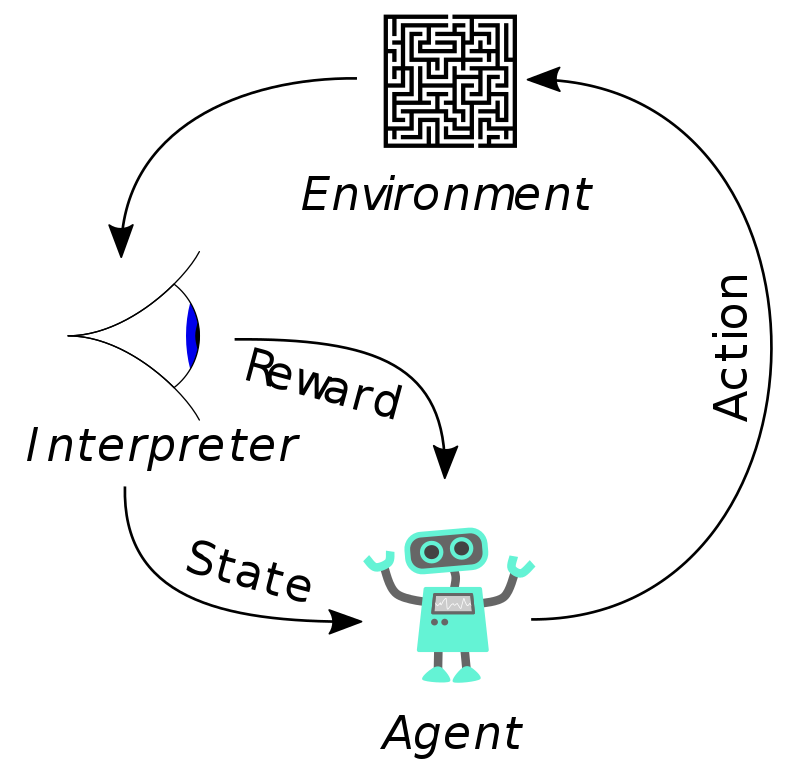
\includegraphics[width=0.7\textwidth]{figures/ml_theory/RL_diagram.png}
	\caption{Reinforcement Learning Diagram}
	\label{fig:rl_diagram}
\end{figure}